% FORMAT AND PACKAGES
% {

% !TEX program = latexmk

\documentclass[a4paper]{article}
\usepackage{a4wide,amssymb,epsfig,latexsym,multicol,array,hhline,fancyhdr}
\usepackage{vntex}
\usepackage{amsmath}
\usepackage{comment}
\usepackage{lastpage}
\usepackage[lined,boxed,commentsnumbered]{algorithm2e}
\usepackage{enumerate}
\usepackage{xcolor}
\usepackage{graphicx}							% Standard graphics package
\usepackage{rotating}
\usepackage{array}
\usepackage{subcaption}
\usepackage{graphicx}
\usepackage{tabularx, caption}
\usepackage{multirow}
\usepackage{caption}
\usepackage{multicol}
\usepackage{rotating}
\usepackage{graphics}
\usepackage{geometry}
\usepackage{setspace}
\usepackage{epsfig}
\usepackage{tikz}
\usepackage{xfrac}
\usepackage{bm}
\usepackage{cite}
\usepackage{enumitem}
\usepackage{parskip}
% code

% landscape page 
\usepackage{lscape}
\usepackage{pdflscape}

%\usepackage[nottoc,numbib]{tocbibind} % Automatically adds bibliography to ToC
\usepackage[colorlinks]{hyperref}
\usepackage[nocomma]{optidef}
\usepackage[table,xcdraw]{xcolor}
\usepackage{float}
% \usepackage[acronym,toc]{glossaries}
% \usepackage[symbols,nogroupskip,nonumberlist]{glossaries-extra}
\usepackage[
 sort=none,% no sorting or indexing required
 abbreviations,% create list of abbreviations
 symbols,% create list of symbols
 stylemods,style=list, % set the default glossary style
 nogroupskip, nonumberlist, nomain
]{glossaries-extra}

% FORMATTING
% {
\DeclareMathOperator{\arccot}{arccot}
\captionsetup[table]{name=Table}
\captionsetup[figure]{name=Figure}
\newenvironment{Description}{\list{}{%
    \let\makelabel\descriptionlabel    % this comes from the original description environment
    \setlength{\rightmargin}{\leftmargin}% this comes from the original quote environment
    \setlength{\labelwidth}{0pt}%          this is new
    }}{\endlist}

%\addbibresource{citations.bib}
    
\hypersetup{urlcolor=blue,linkcolor=black,citecolor=black,colorlinks=true} 
\usetikzlibrary{arrows,snakes,backgrounds}
\definecolor{mathblue}{RGB}{0,114,188}
% \makeatletter  \def\m@th{\mathsurround\z@\color{mathblue}} \makeatother
% \everymath{\color{mathblue}}
% \setmathfont[Color=000000]{Arial}
%\usepackage{pstcol} 								% PSTricks with the standard color package
\newtheorem{theorem}{{\bf Theorem}}
\newtheorem{property}{{\bf Property}}
\newtheorem{proposition}{{\bf Proposition}}
\newtheorem{corollary}[proposition]{{\bf Corollary}}
\newtheorem{lemma}[proposition]{{\bf Lemma}}

\AtBeginDocument{\renewcommand{\listfigurename}{Danh sách hình ảnh}}
\AtBeginDocument{\renewcommand{\listtablename}{Danh sách bảng}}
\AtBeginDocument{\renewcommand*\contentsname{Mục lục}}
\AtBeginDocument{\renewcommand*\refname{Tham khảo}}
%\usepackage{fancyhdr}

\setlength{\headheight}{40pt}
\pagestyle{fancy}
\fancyhead{} % clear all header fields
\fancyhead[L]{
 \begin{tabular}{rl}
    \begin{picture}(25,15)(0,0)
    \put(0,-8){
\includegraphics[width=8mm, height=8mm]{image/logo.png}}
    %\put(0,-8){\epsfig{width=10mm,figure=hcmut.eps}}
   \end{picture}&
	%\includegraphics[width=8mm, height=8mm]{hcmut.png} & %
	\begin{tabular}{l}
		\textbf{\bf \ttfamily Trường Đại học Bách khoa Thành phố Hồ Chí Minh}\\
		\textbf{\bf \ttfamily Khoa Khoa học và Kỹ thuật Máy tính}
	\end{tabular} 	
 \end{tabular}
}
\fancyhead[R]{
	\begin{tabular}{l}
		\tiny \bf \\
		\tiny \bf 
	\end{tabular}  }
\fancyfoot{} % clear all footer fields
\fancyfoot[L]{\scriptsize \ttfamily Đồ án tổng hợp hướng CNPM - Năm học 2025 - 2026}
\fancyfoot[R]{\scriptsize \ttfamily Trang {\thepage}/\pageref{LastPage}}
\renewcommand{\headrulewidth}{0.3pt}
\renewcommand{\footrulewidth}{0.3pt}
\captionsetup[table]{name=Bảng}
\captionsetup[figure]{name=Hình}

\setcounter{secnumdepth}{4}
\setcounter{tocdepth}{4}

\makeatletter
\newcounter {subsubsubsection}[subsubsection]
\renewcommand\thesubsubsubsection{\thesubsubsection .\@alph\c@subsubsubsection}
\newcommand\subsubsubsection{\@startsection{subsubsubsection}{4}{\z@}%
                                     {-3.25ex\@plus -1ex \@minus -.2ex}%
                                     {1.5ex \@plus .2ex}%
                                     {\normalfont\normalsize\bfseries}}
\newcommand*\l@subsubsubsection{\@dottedtocline{3}{7.0em}{4.1em}}
\newcommand*{\subsubsubsectionmark}[1]{}
% \def\m@th{\mathsurround\z@\color{mathblue}}
\makeatother
% }
% }

% ACRONYMS & SYMBOLS
% {
% \makeglossaries
\setabbreviationstyle{long-short}
\newabbreviation{csp}{CSP}{Cutting Stock Problem (Bài toán cắt vật tư)}
\newabbreviation{lp}{LP}{Linear Programming (Quy hoạch tuyến tính)}
\newabbreviation{ilp}{ILP}{Integer Linear Programming (Quy hoạch tuyến tính nguyên)}
\newabbreviation{bb}{B\&B}{Branch and Bound Method (Phương pháp nhánh và cận)}
\newabbreviation{np}{NP}{
Nondeterministic polynomial time (Bất định trong thời gian đa thức)}

% \glsnoexpandfields
% \glsxtrnewsymbol[description = {Tập hợp số tự nhiên}]{natural}{\ensuremath{\mathbb{N}}}
 \glsxtrnewsymbol[description = {Tập hợp số thực}]{real}{\ensuremath{\mathbb{R}}}
\glsxtrnewsymbol[description = {Tập hợp số nguyên dương}]{real_positive}{\ensuremath{\mathbb{Z}^+}}
\setlength\parindent{24pt}
% }

\makeatletter
\def\magicomadjust{0em}  % a way to adjust if the spacing should be different
\newdimen\indent@amount
\def\magicom{\relax
  \ifhmode $$%
    \predisplaypenalty\@M \postdisplaypenalty\@M
    \abovedisplayskip-\baselineskip \belowdisplayskip\z@
    \abovedisplayshortskip\abovedisplayskip
    \belowdisplayshortskip\belowdisplayskip
    \global\indent@amount\predisplaysize
     $$\count@\prevgraf \advance\count@-\thr@@
         \prevgraf\count@
    \global\advance\indent@amount-2em  % correction for \predisplaysize indent
    \global\advance\indent@amount\magicomadjust  % correction for verse env, for example
    \hspace*\indent@amount
  \else\typeout{*Not in hmode*}\fi}
\makeatother

\renewcommand*\contentsname{Mục lục}
\renewcommand{\arraystretch}{1.5}\renewcommand{\arraystretch}{1.4}

\newenvironment{blockquote}{%
  \par%
  \medskip
  \leftskip=2.5em%
  \noindent\ignorespaces}{%
  \par\medskip
}
\setlength{\parindent}{0pt} % Forces no indent for the whole document
% DOCUMENT
\begin{document}

% TITLE PAGE
\begin{titlepage}
\begin{center}
\large{ĐẠI HỌC QUỐC GIA THÀNH PHỐ HỒ CHÍ MINH} \\
TRƯỜNG ĐẠI HỌC BÁCH KHOA \\
KHOA KHOA HỌC VÀ KỸ THUẬT MÁY TÍNH
\end{center}

\vspace{1cm}

\begin{figure}[h!]
\begin{center}

\includegraphics[width=3cm]{image/logo.png}
\end{center}
\end{figure}

\vspace{0.8cm}


\begin{center}
\begin{tabular}{c}
\multicolumn{1}{l}{\textbf{{\Large ĐỒ ÁN TỔNG HỢP HƯỚNG CNPM (CO3103)}}}\\
~~\\
\hline
\\
\multicolumn{1}{l}{\textbf{{Báo cáo Đồ án tổng hợp}}}\\
\\
\textbf{\textit{{\huge Seven Deadly Sins}}}\\
\textbf{\textit{{\huge }}}\\
\\
\hline
\end{tabular}
\end{center}

\vspace{0.2cm}
\begin{center}
Giảng viên hướng dẫn:  Mai Đức Trung\\
\vspace{0.7cm}
\begin{tabular}{|c|c|c|c|}
\hline
\textbf{STT} & \textbf{Họ tên SV} & \textbf{MSSV} & \textbf{Lớp} \\
\hline 
%%%%%Student 1%%%%%%%%%%
{1} & {Nguyễn Đức Nghĩa}& {2312266} & {L03}\\
 
\hline 
%%%%%Student 2%%%%%%%%%%%
{2} & {Trần Tiến Khải} & {2311566} & {L03}\\

\hline
%%%%%Student 3%%%%%%%%%%%
{3} & {Phan Huy Quang Minh} & {2312105} & {L03} \\

\hline
%%%%%Student %%%%%%%%%%%
{4} & {Hà Cao Đức Minh} & {2312059} & {L02} \\

\hline
%%%%%Student %%%%%%%%%%%
{5} & {Trần Quốc Toàn} & {2213504} & {L03} \\

\hline
%%%%%Student %%%%%%%%%%%
{6} & {Nguyễn Vũ Tường} & {2313834} & {L03} \\
\hline

\end{tabular}

\vfill
Thành phố Hồ Chí Minh, năm 2025

\end{center}
\end{titlepage}

\pagebreak
\tableofcontents
\pagebreak

\addcontentsline{toc}{section}{Danh sách thành viên và khối lượng công việc}

\begin{center}
\begin{table}[H]
\centering
\renewcommand{\arraystretch}{1.5}
\begin{tabular}{|c|c|c|c|}
\hline
\textbf{STT} & \textbf{Họ và tên} & \textbf{MSSV} & \textbf{\% hoàn thành}\\
\hline 
%%%%%Student 1%%%%%%%%%%
\multirow{1}{*}{1} & \multirow{1}{*}{Nguyễn Đức Nghĩa} & \multirow{1}{*}{2312266} & \multirow{1}{*}{100\%}\\
\hline 
%%%%%Student 6%%%%%%%%%%%
\multirow{1}{*}{2} & \multirow{1}{*}{Trần Tiến Khải} & \multirow{1}{*}{2311566} & \multirow{1}{*}{100\%}\\
\hline
%%%%%Student 2%%%%%%%%%%%
\multirow{1}{*}{3} & \multirow{1}{*}{Phan Huy Quang Minh} & \multirow{1}{*}{2312105} & \multirow{1}{*}{100\%}\\
\hline
%%%%%Student 4%%%%%%%%%%%
\multirow{1}{*}{4} & \multirow{1}{*}{Hà Cao Đức Minh} & \multirow{1}{*}{2312059} & \multirow{1}{*}{100\%}\\
\hline
%%%%%Student 5%%%%%%%%%%%
\multirow{1}{*}{5} & \multirow{1}{*}{Trần Quốc Toàn} & \multirow{1}{*}{2213504} & \multirow{1}{*}{100\%}\\
\hline
%%%%%Student 3%%%%%%%%%%%
\multirow{1}{*}{6} & \multirow{1}{*}{Nguyễn Vũ Tường} & \multirow{1}{*}{2313834} & \multirow{1}{*}{100\%}\\
\hline

\end{tabular}
\end{table}
\end{center}
% Glossaries
% {}

% }

\include{Introduction_Acknowledge}
\input{DevelopmentOrientation}
\input{Requirement}
\input{Usecase}
\section{Lược đồ lớp hiện thực và đặc tả các lớp}

\begin{figure}[h] 
    \centering
    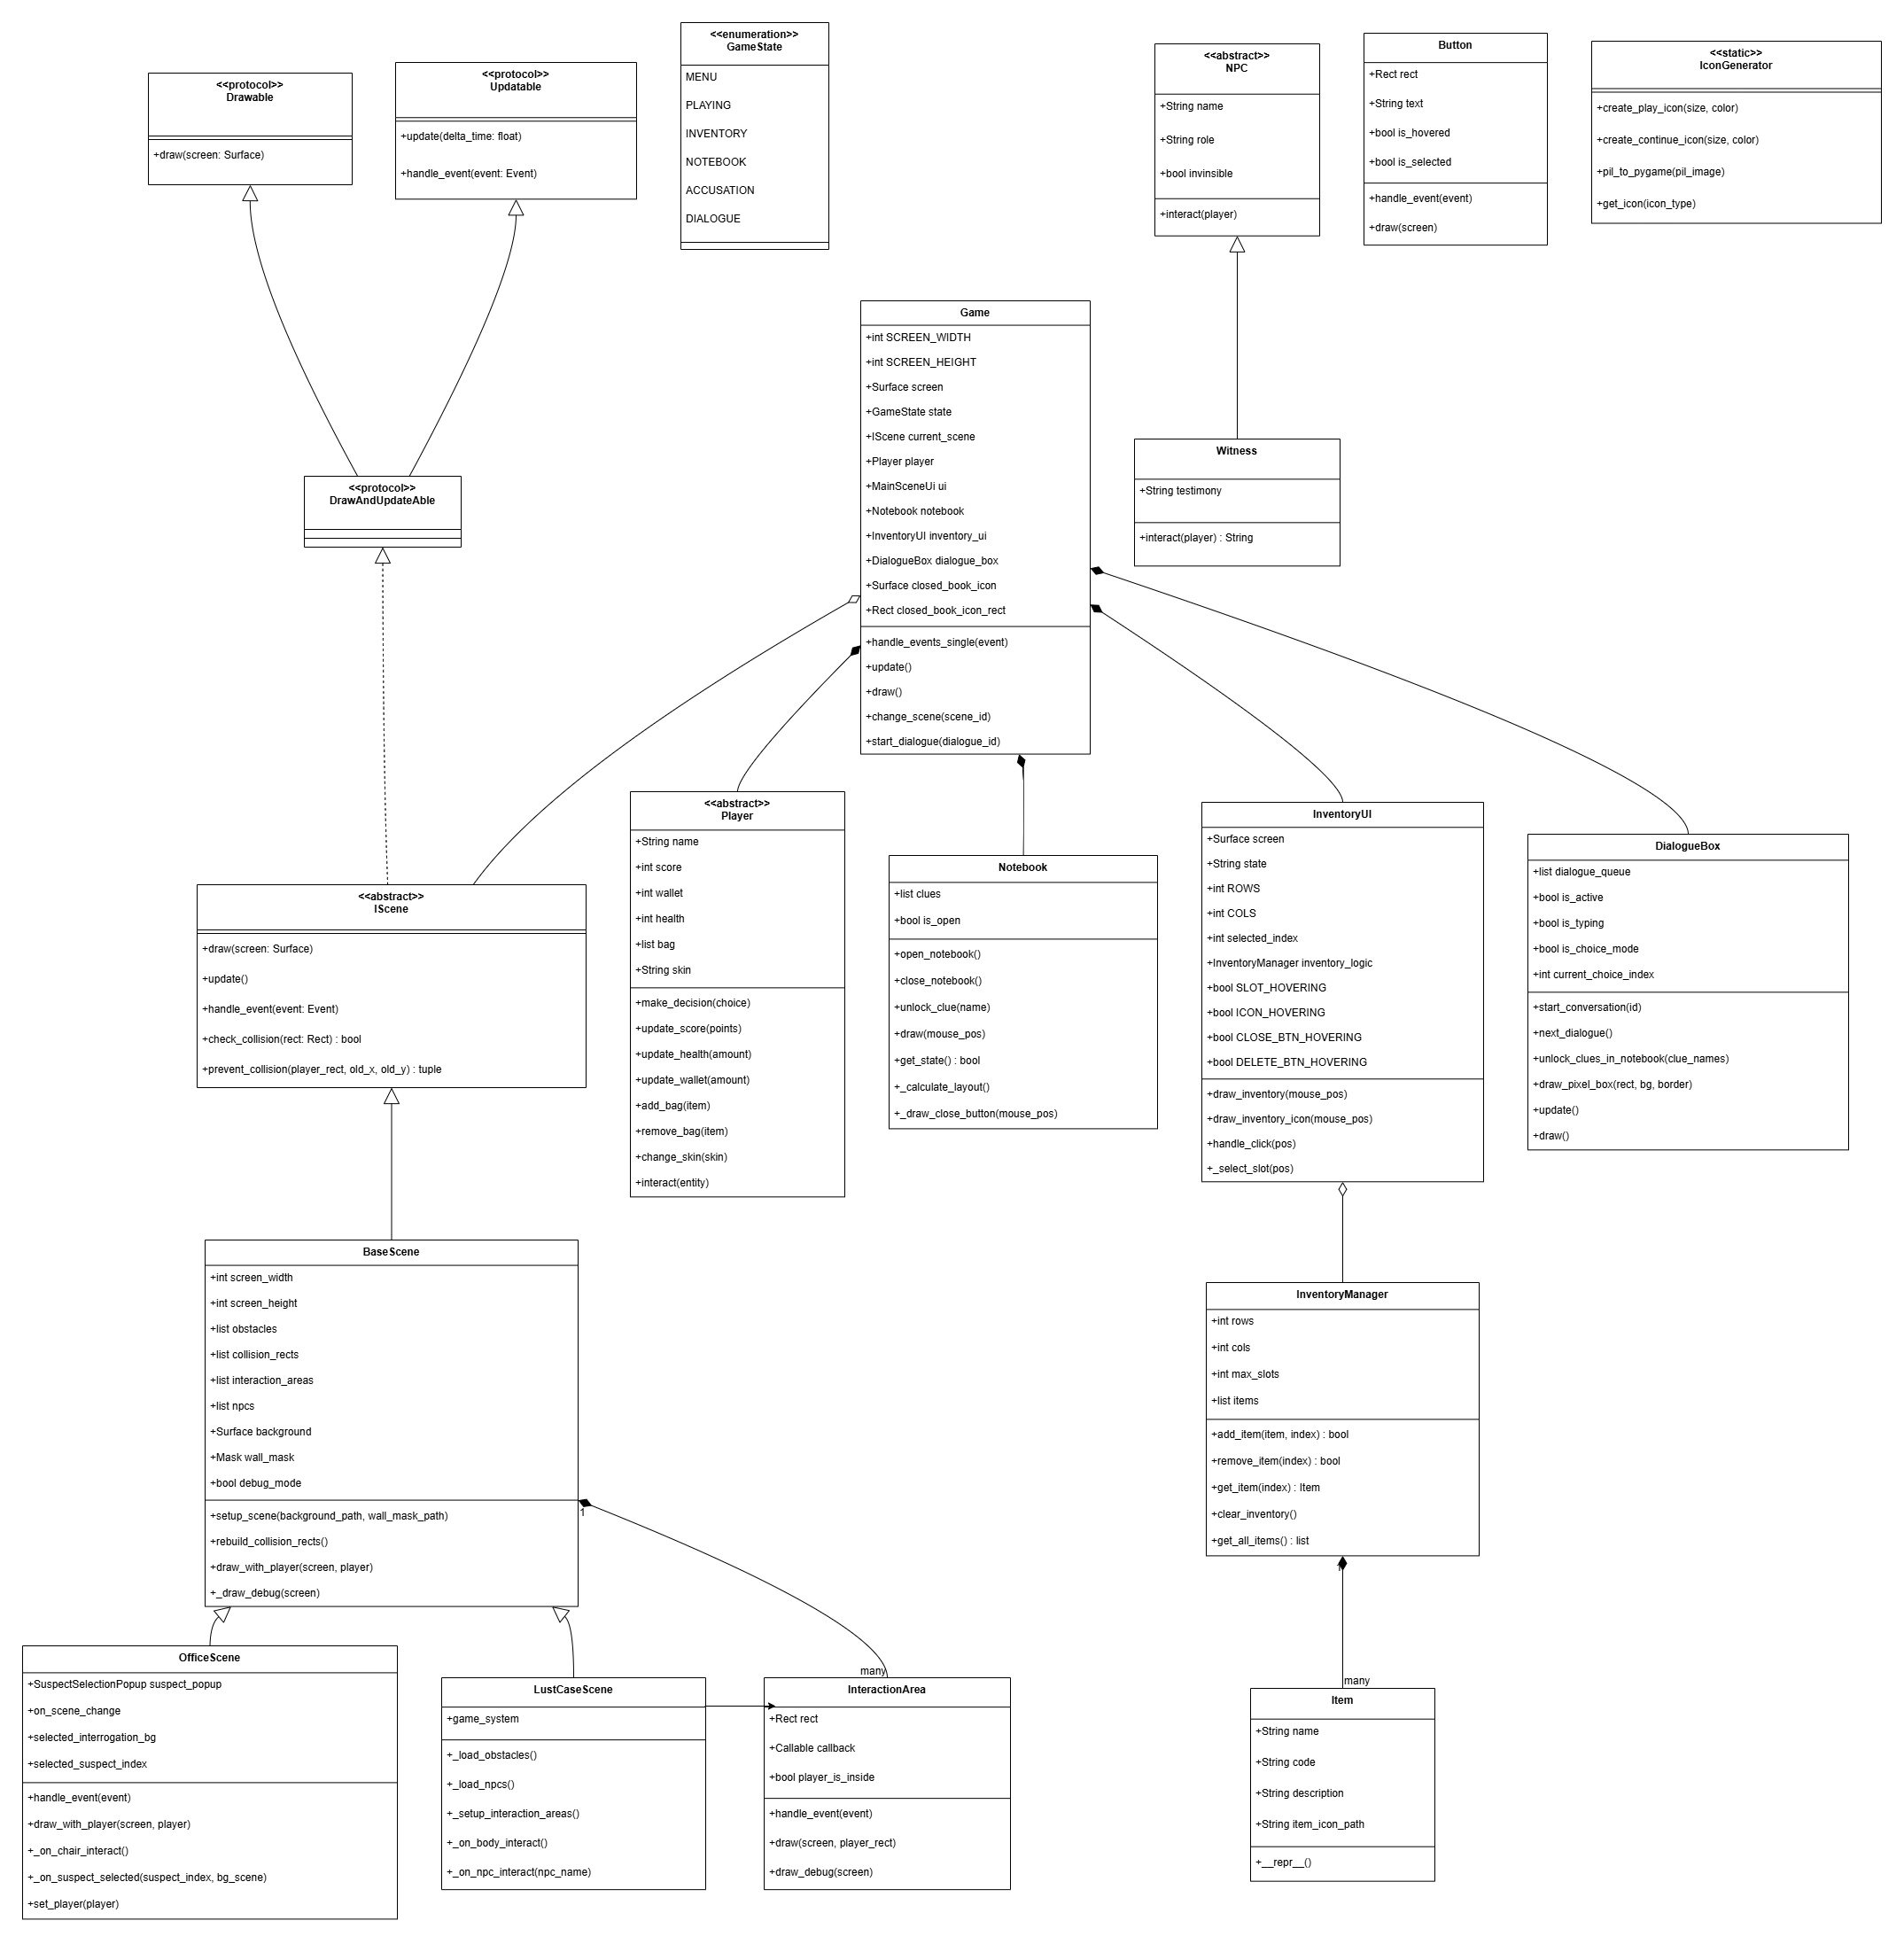
\includegraphics[width=\textwidth]{image/Diagram/Class.png} 
\end{figure}

\begin{description}

    \item[Lớp: Game] 
    Lớp trung tâm điều phối toàn bộ vòng lặp trò chơi (vẽ, cập nhật, xử lý sự kiện). Quản lý các thành phần chính như người chơi, cảnh hiện tại và chuyển đổi trạng thái giao diện.
    \begin{itemize}
        \item \textbf{handle\_events\_single(event) : void} \\
        Xử lý các sự kiện đầu vào (chuột, bàn phím) và phân luồng dựa trên trạng thái \texttt{GameState}.
        \item \textbf{change\_scene(scene\_id) : void} \\
        Thực hiện chuyển đổi giữa các màn chơi khác nhau và khởi tạo lại các tham chiếu cần thiết cho cảnh mới.
        \item \textbf{start\_dialogue(id) : void} \\
        Kích hoạt hệ thống hội thoại và nạp dữ liệu từ tệp cấu hình hội thoại.
    \end{itemize}

    \item[Lớp: BaseScene (Abstract)]
    Lớp trừu tượng cung cấp khung làm việc cơ bản cho mọi cảnh trong game, bao gồm quản lý hình ảnh nền và hệ thống va chạm.
    \begin{itemize}
        \item \textbf{setup\_scene(background, mask) : void} \\
        Tải tài nguyên hình ảnh nền và bản đồ va chạm (mask) để ngăn nhân vật đi xuyên tường.
        \item \textbf{draw\_with\_player(screen, player) : void} \\
        Vẽ cảnh và nhân vật theo thứ tự ưu tiên trục Y (Y-sorting) để tạo hiệu ứng chiều sâu 2D.
    \end{itemize}

    \item[Lớp: Notebook]
    Quản lý sổ tay ghi chép thám tử, lưu trữ và hiển thị các manh mối đã được người chơi thu thập.
    \begin{itemize}
        \item \textbf{unlock\_clue(name) : void} \\
        Tìm kiếm manh mối trong cơ sở dữ liệu và thay đổi trạng thái từ khóa sang hiển thị (\texttt{unlocked}).
        \item \textbf{\_calculate\_layout() : void} \\
        Tính toán vị trí các dòng chữ để nội dung luôn nằm khớp trên các đường kẻ của trang giấy trong sổ tay.
    \end{itemize}

    \item[Lớp: InventoryManager]
    Quản lý logic túi đồ, chịu trách nhiệm lưu trữ và thao tác trên mảng dữ liệu các vật phẩm.
    \begin{itemize}
        \item \textbf{add\_item(item, index) : bool} \\
        Thêm vật phẩm vào một ô cụ thể hoặc tìm ô trống đầu tiên. Trả về thành công hoặc thất bại.
        \item \textbf{remove\_item(index) : bool} \\
        Xóa dữ liệu vật phẩm tại vị trí được chỉ định để giải phóng ngăn chứa.
    \end{itemize}

    \item[Lớp: DialogueBox]
    Xử lý hiển thị hộp thoại, hiệu ứng chữ chạy và quản lý các lựa chọn của người chơi trong tương tác NPC.
    \begin{itemize}
        \item \textbf{next\_dialogue() : void} \\
        Chuyển sang đoạn thoại tiếp theo hoặc hiển thị danh sách lựa chọn nếu nhánh thoại kết thúc.
        \item \textbf{draw\_pixel\_box(rect, bg, border) : void} \\
        Vẽ hộp hội thoại theo phong cách Pixel Art với viền vàng và hiệu ứng đổ bóng đặc trưng.
    \end{itemize}

    \item[Lớp: InteractionArea]
    Định nghĩa một vùng không gian mà người chơi có thể tương tác khi đứng bên trong.
    \begin{itemize}
        \item \textbf{handle\_event(event) : void} \\
        Kiểm tra nếu người chơi nhấn phím \texttt{[F]} khi đang đứng trong vùng tương tác để kích hoạt hàm callback.
        \item \textbf{draw(screen, player\_rect) : void} \\
        Hiển thị chỉ dẫn tương tác lơ lửng phía trên đầu của nhân vật khi họ đi vào vùng này.
    \end{itemize}

\end{description}
\section{Mockup Giao Diện}

\subsection{Giao diện chính và Bối cảnh}

% Nhóm 1: Main Menu và Scene (Trang chính và bối cảnh game)
\begin{figure}[H]
    \centering
    % Hàng 1
    \begin{minipage}{0.45\textwidth}
        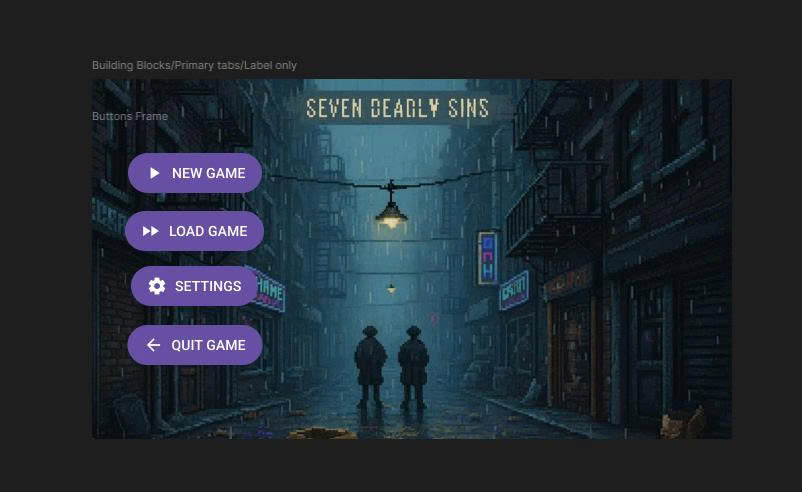
\includegraphics[width=\textwidth]{image/Mockup UI/Main Menu.jpg}
        \caption*{Main Menu}
    \end{minipage}
    \hfill
    \begin{minipage}{0.45\textwidth}
        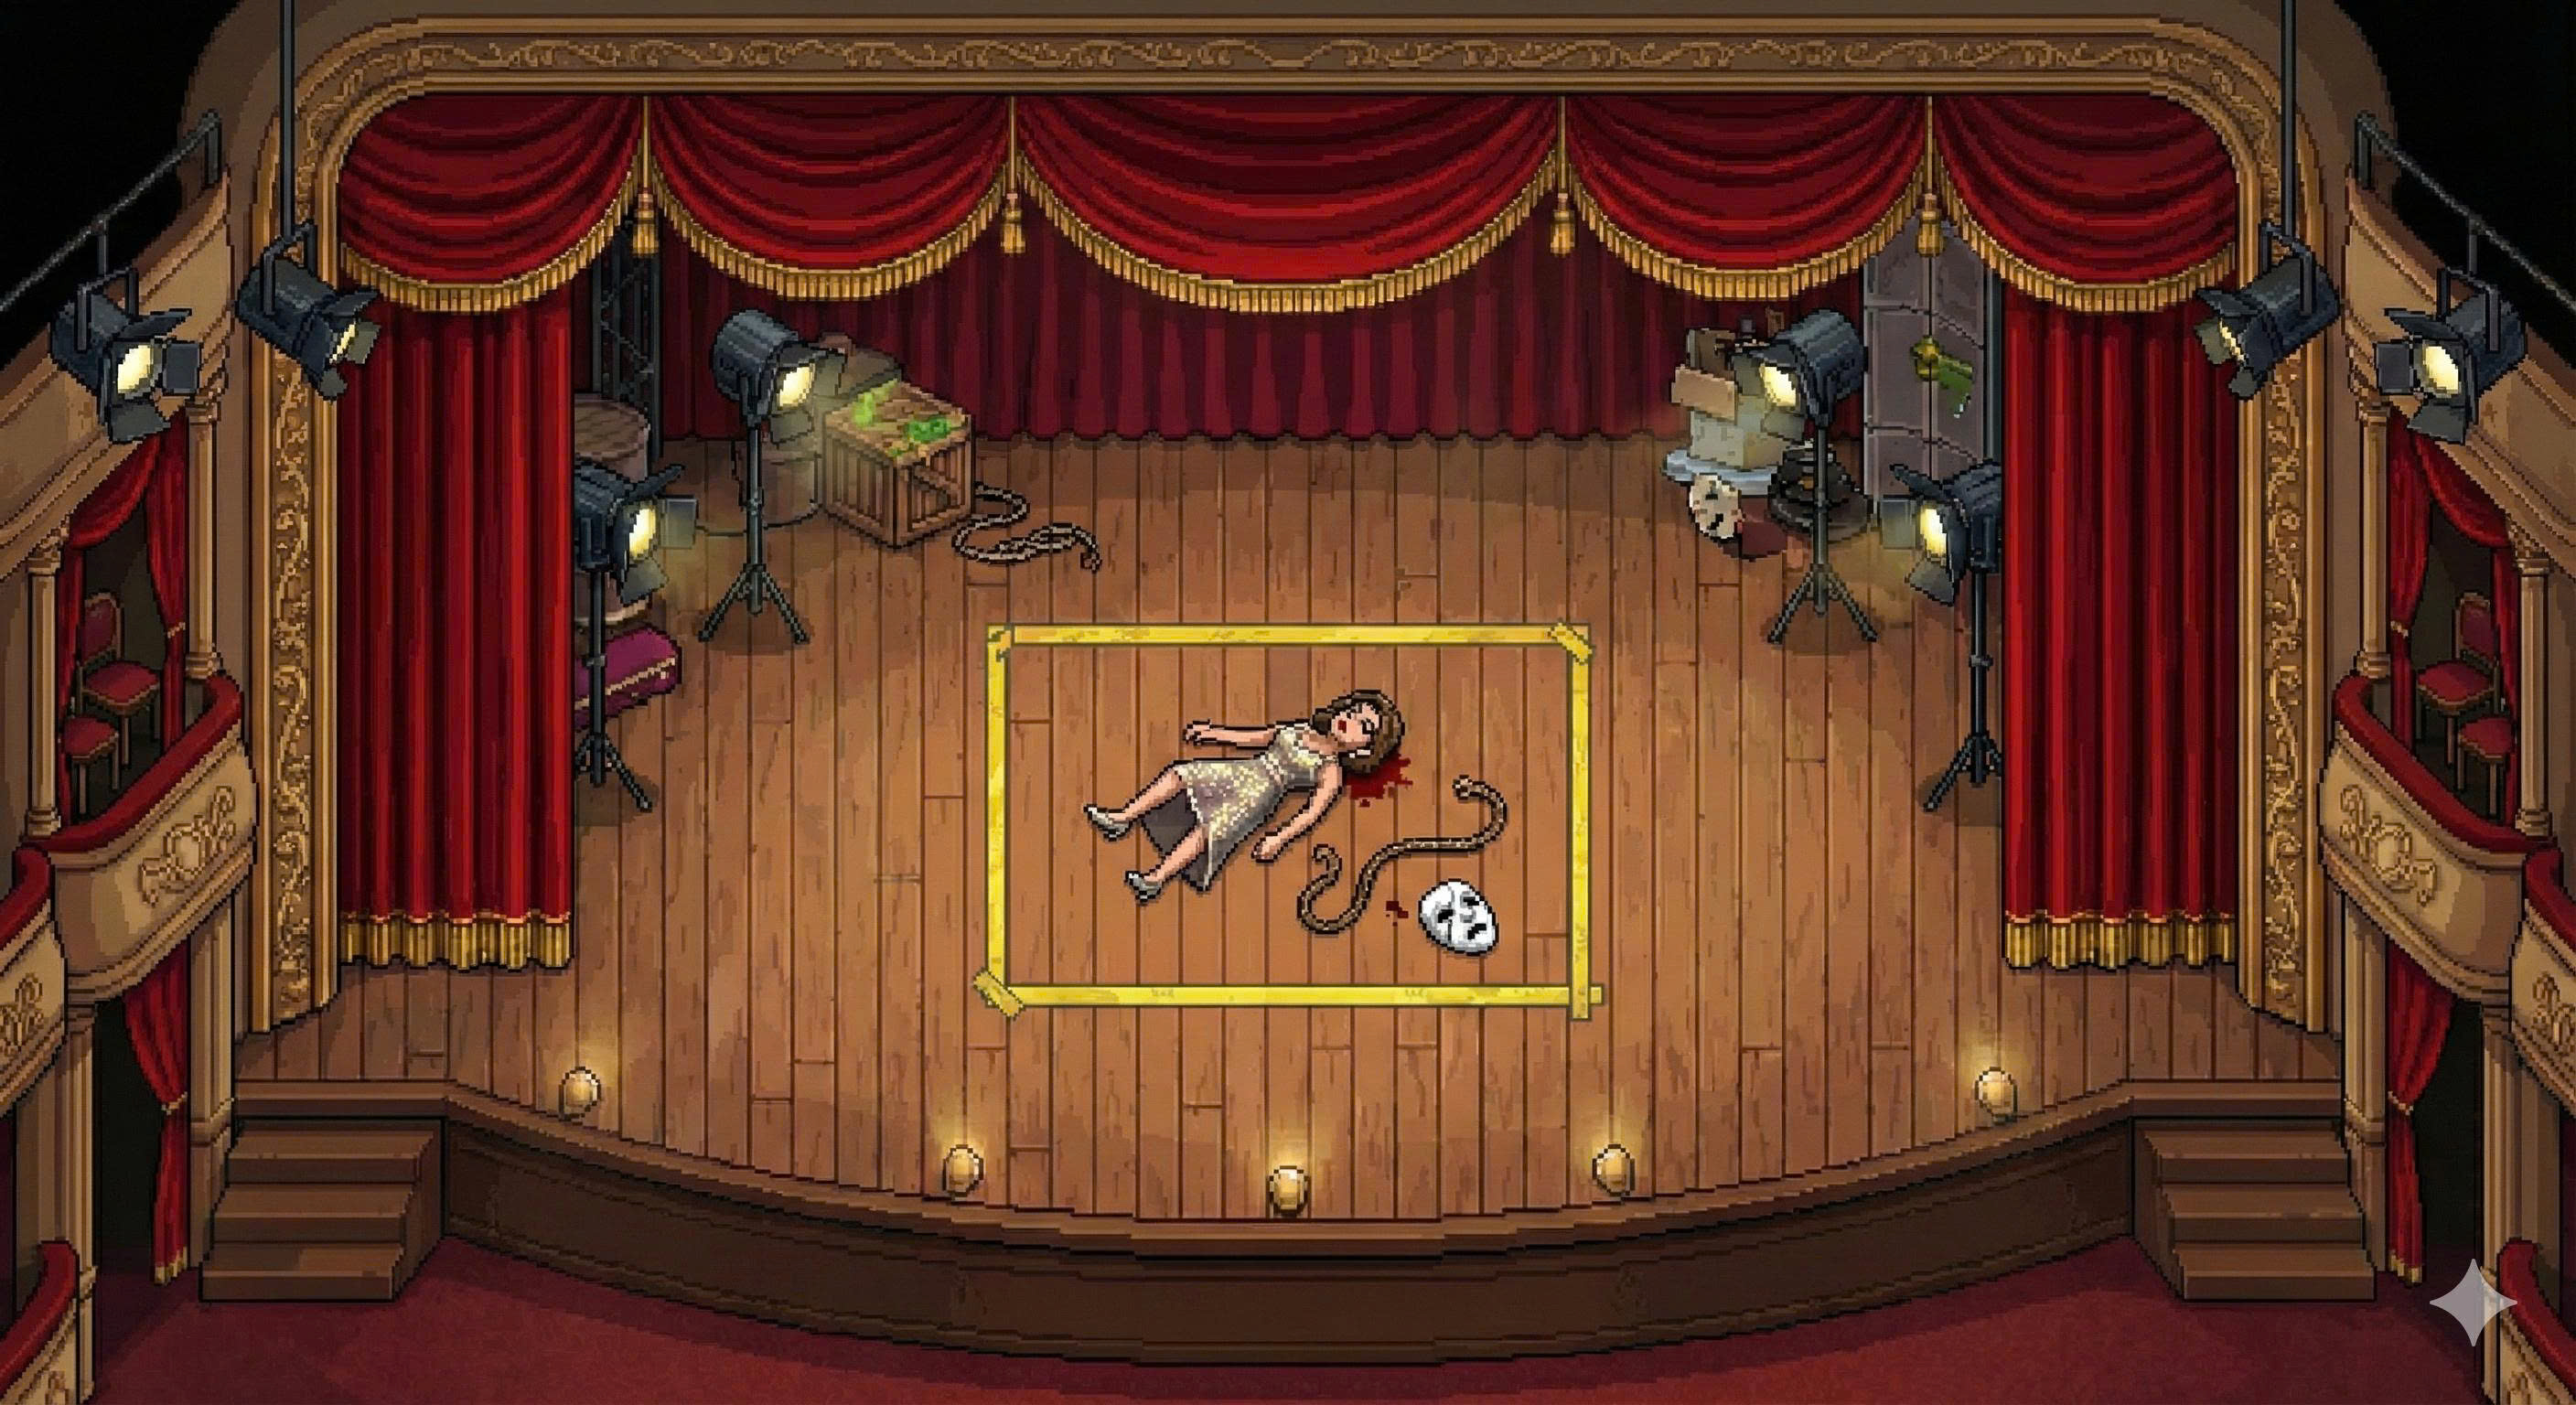
\includegraphics[width=\textwidth]{image/Mockup UI/Scene.jpg}
        \caption*{Game Scene}
    \end{minipage}

    \vspace{0.5cm}

    % Hàng 2
    \begin{minipage}{0.45\textwidth}
        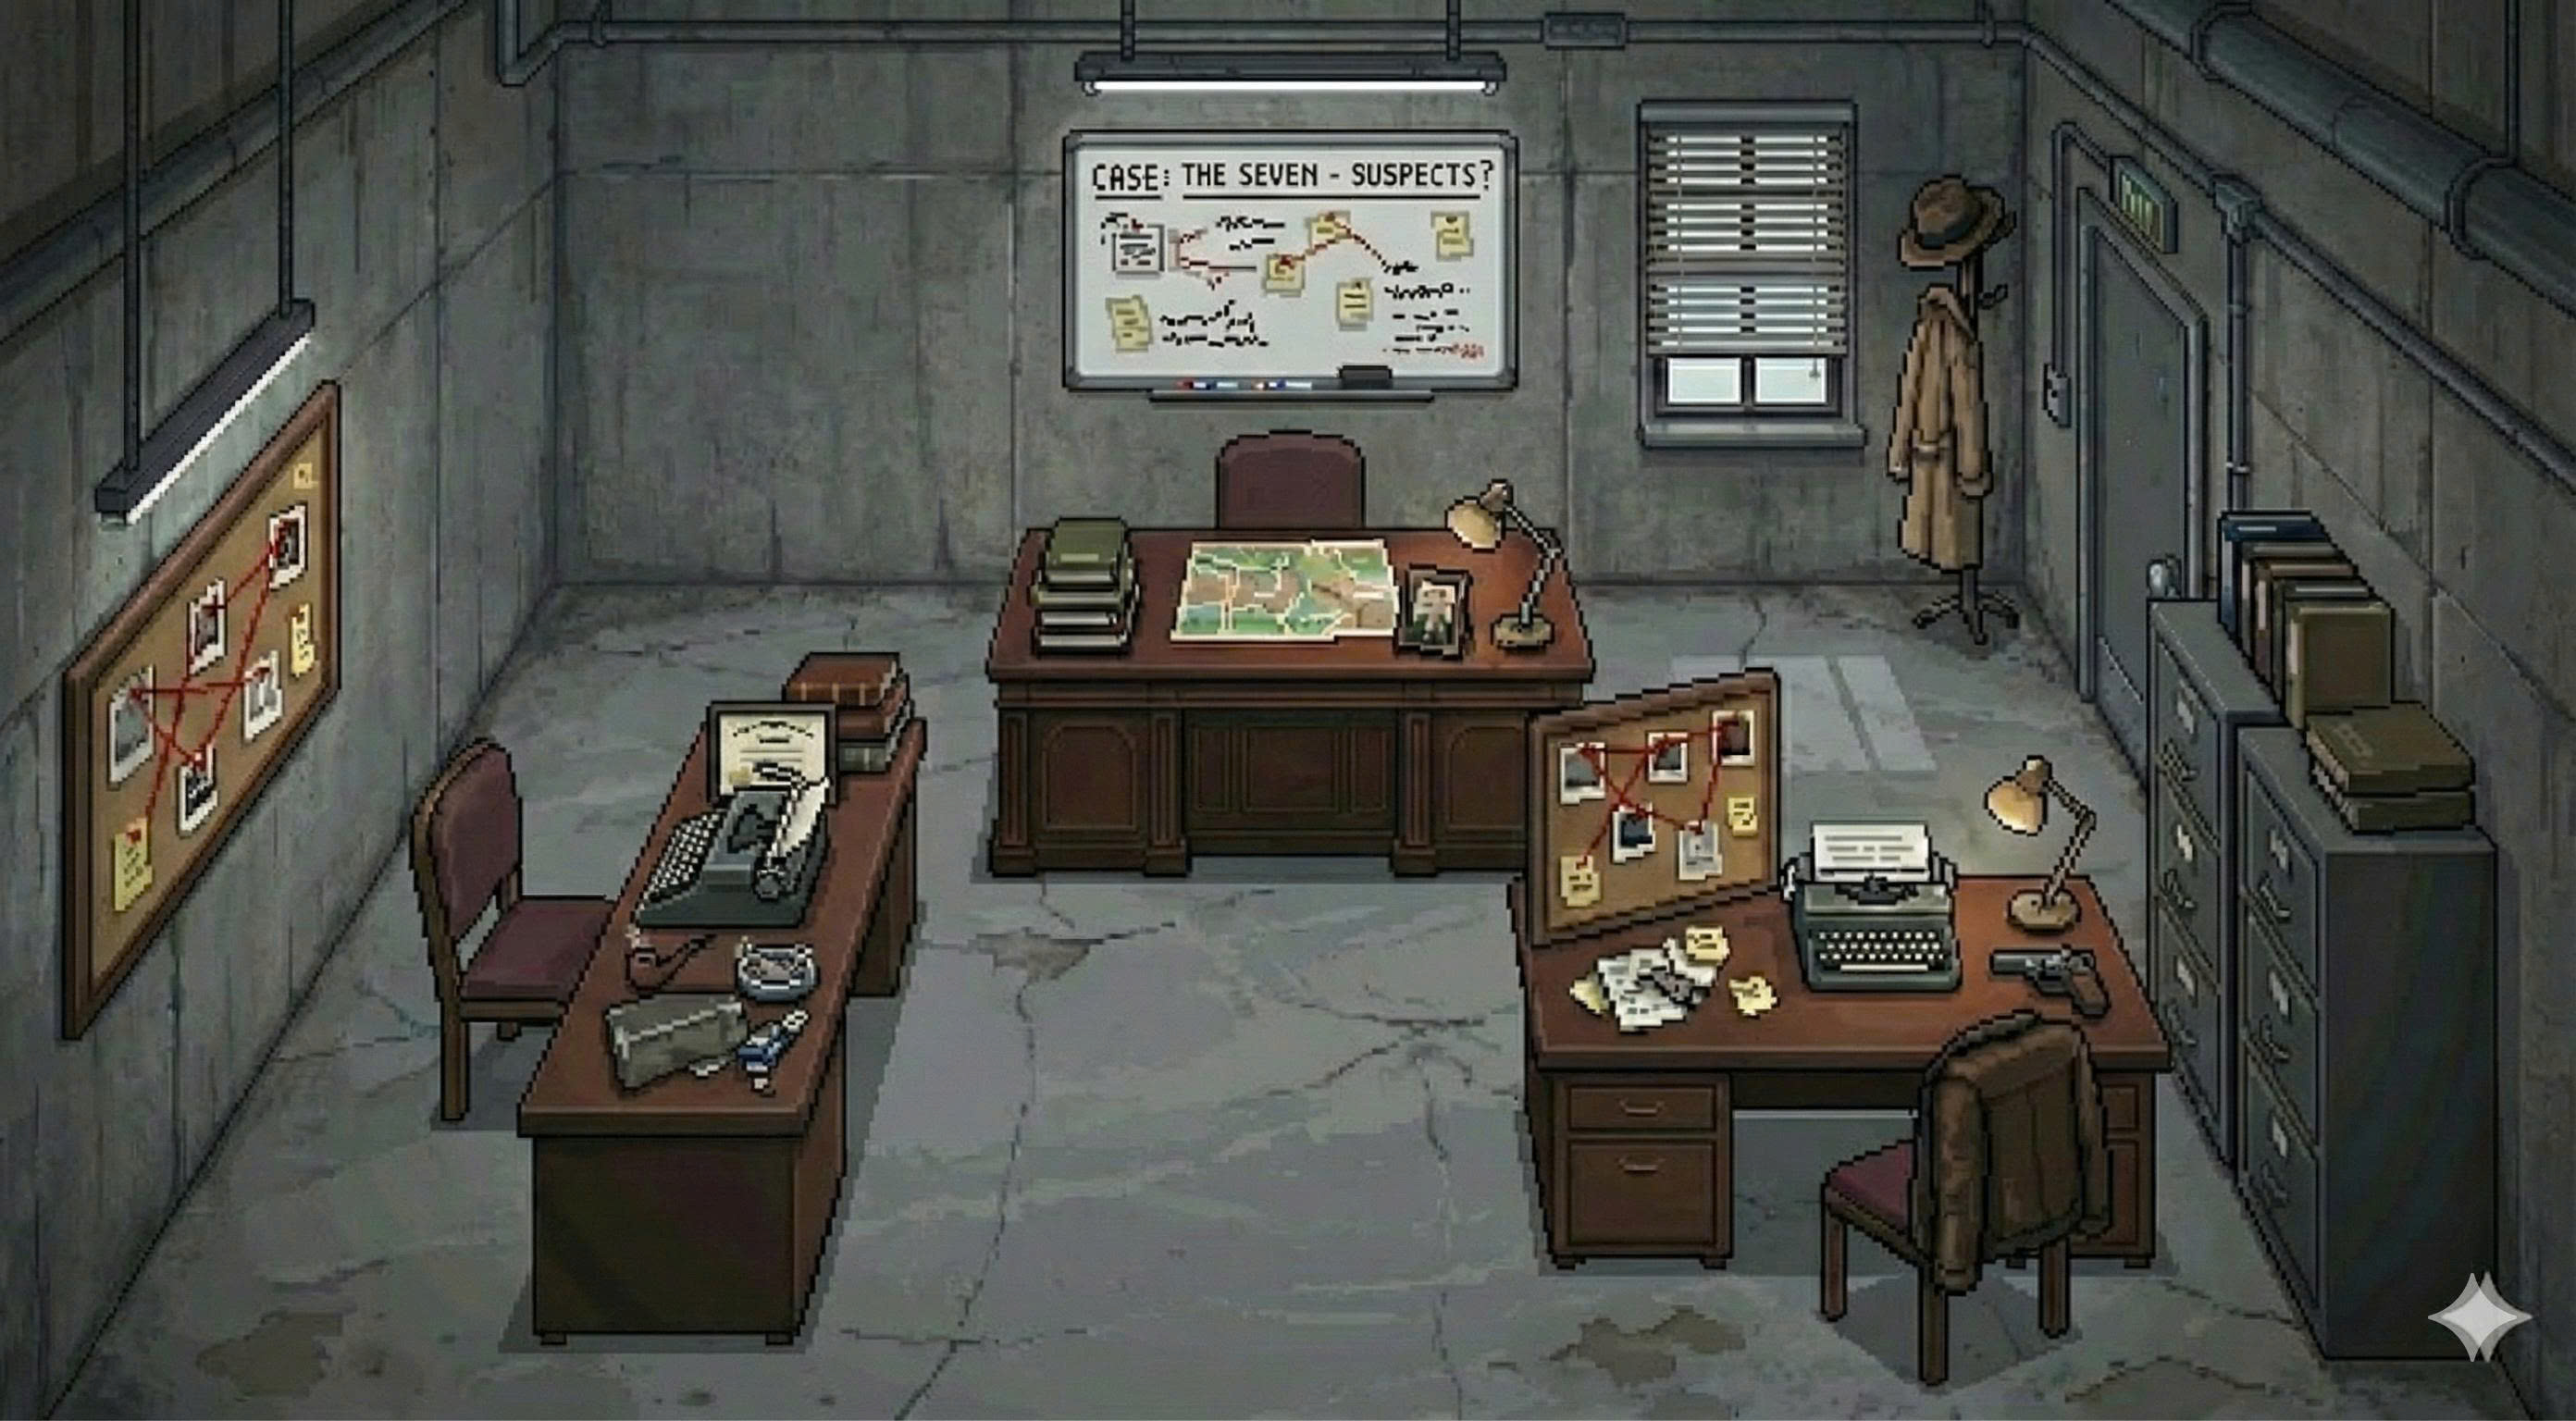
\includegraphics[width=\textwidth]{image/Mockup UI/Office.jpg}
        \caption*{Office Background}
    \end{minipage}
    \hfill
    \begin{minipage}{0.45\textwidth}
        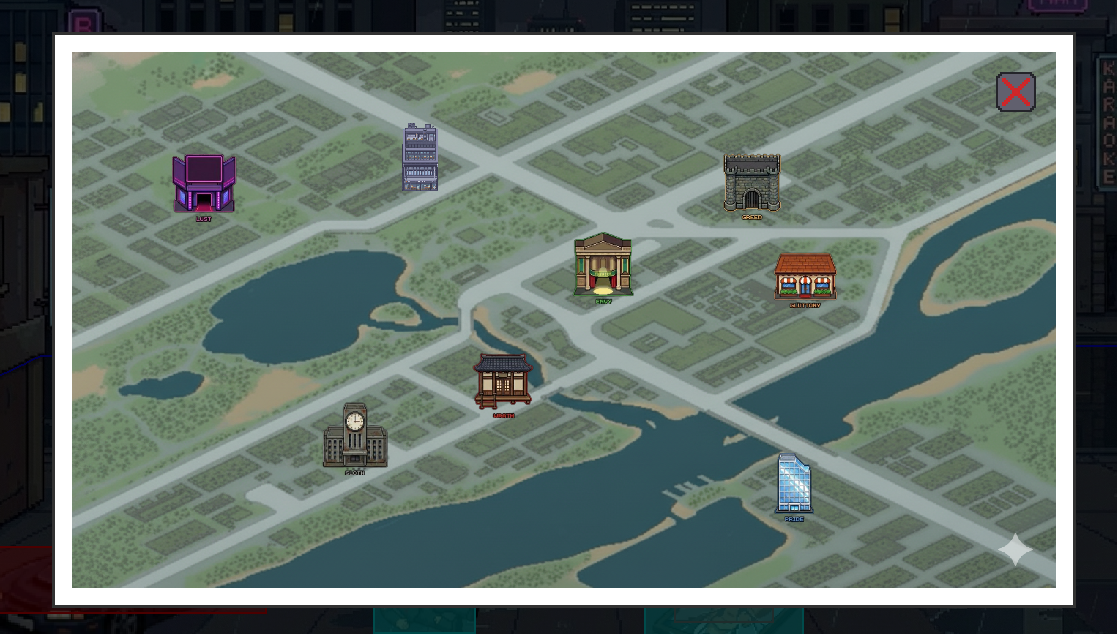
\includegraphics[width=\textwidth]{image/Mockup UI/Map.png}
        \caption*{World Map}
    \end{minipage}
\end{figure}
\clearpage

\subsection{Giao diện Chức năng (Gameplay UI)}

% Nhóm 2: Inventory và Notebook (Hệ thống túi đồ và ghi chép)
\begin{figure}[H]
    \centering
    % Hàng 1
    \begin{minipage}{0.45\textwidth}
        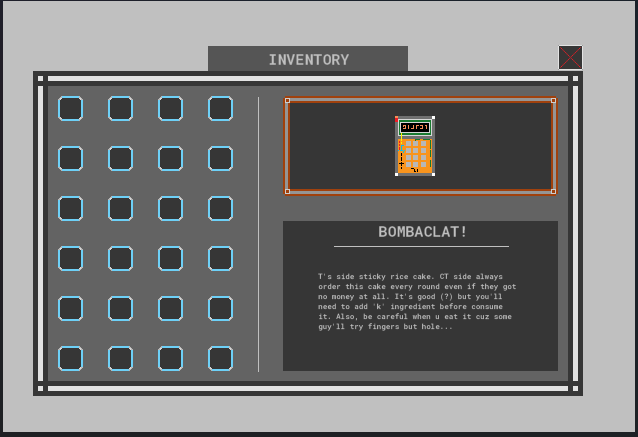
\includegraphics[width=\textwidth]{image/Mockup UI/InventoryO.png}
        \caption*{Inventory Old}
    \end{minipage}
    \hfill
    \begin{minipage}{0.45\textwidth}
        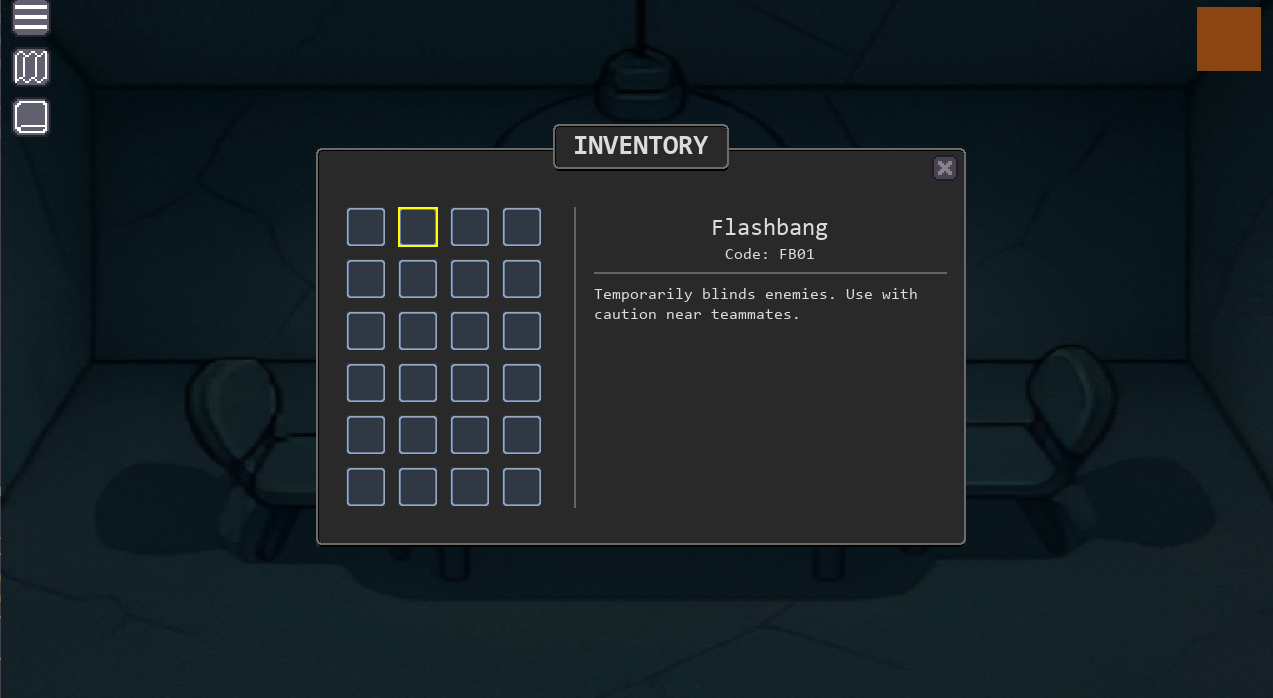
\includegraphics[width=\textwidth]{image/Mockup UI/Inventory.png}
        \caption*{Inventory New}
    \end{minipage}

    \vspace{0.5cm}

    % Hàng 2
    \begin{minipage}{0.45\textwidth}
        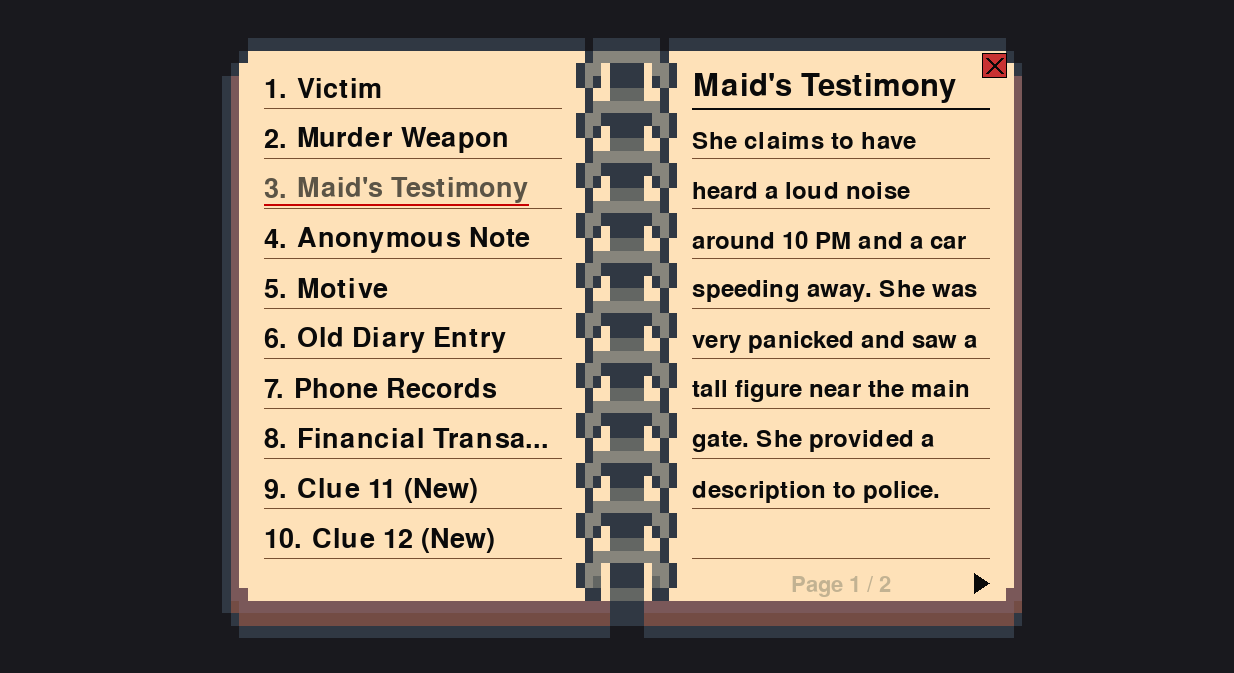
\includegraphics[width=\textwidth]{image/Mockup UI/Notebook.png}
        \caption*{Notebook System}
    \end{minipage}
    \hfill
    \begin{minipage}{0.45\textwidth}
        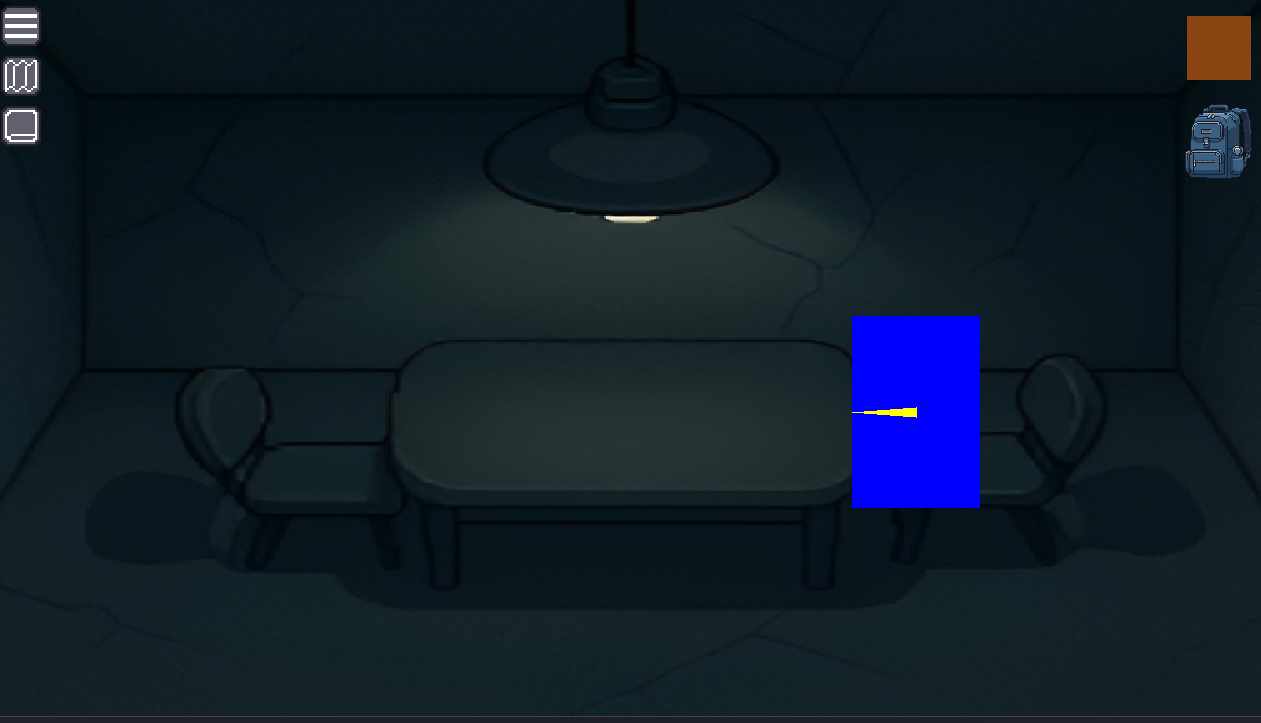
\includegraphics[width=\textwidth]{image/Mockup UI/Iter.png}
        \caption*{Interaction UI}
    \end{minipage}
\end{figure}
\clearpage

\subsection{Nhân vật và tương tác}

% Nhóm 3: Player và Accuse (Nhân vật và tính năng buộc tội)
\begin{figure}[H]
    \centering
    % Hàng 1
    \begin{minipage}{0.45\textwidth}
        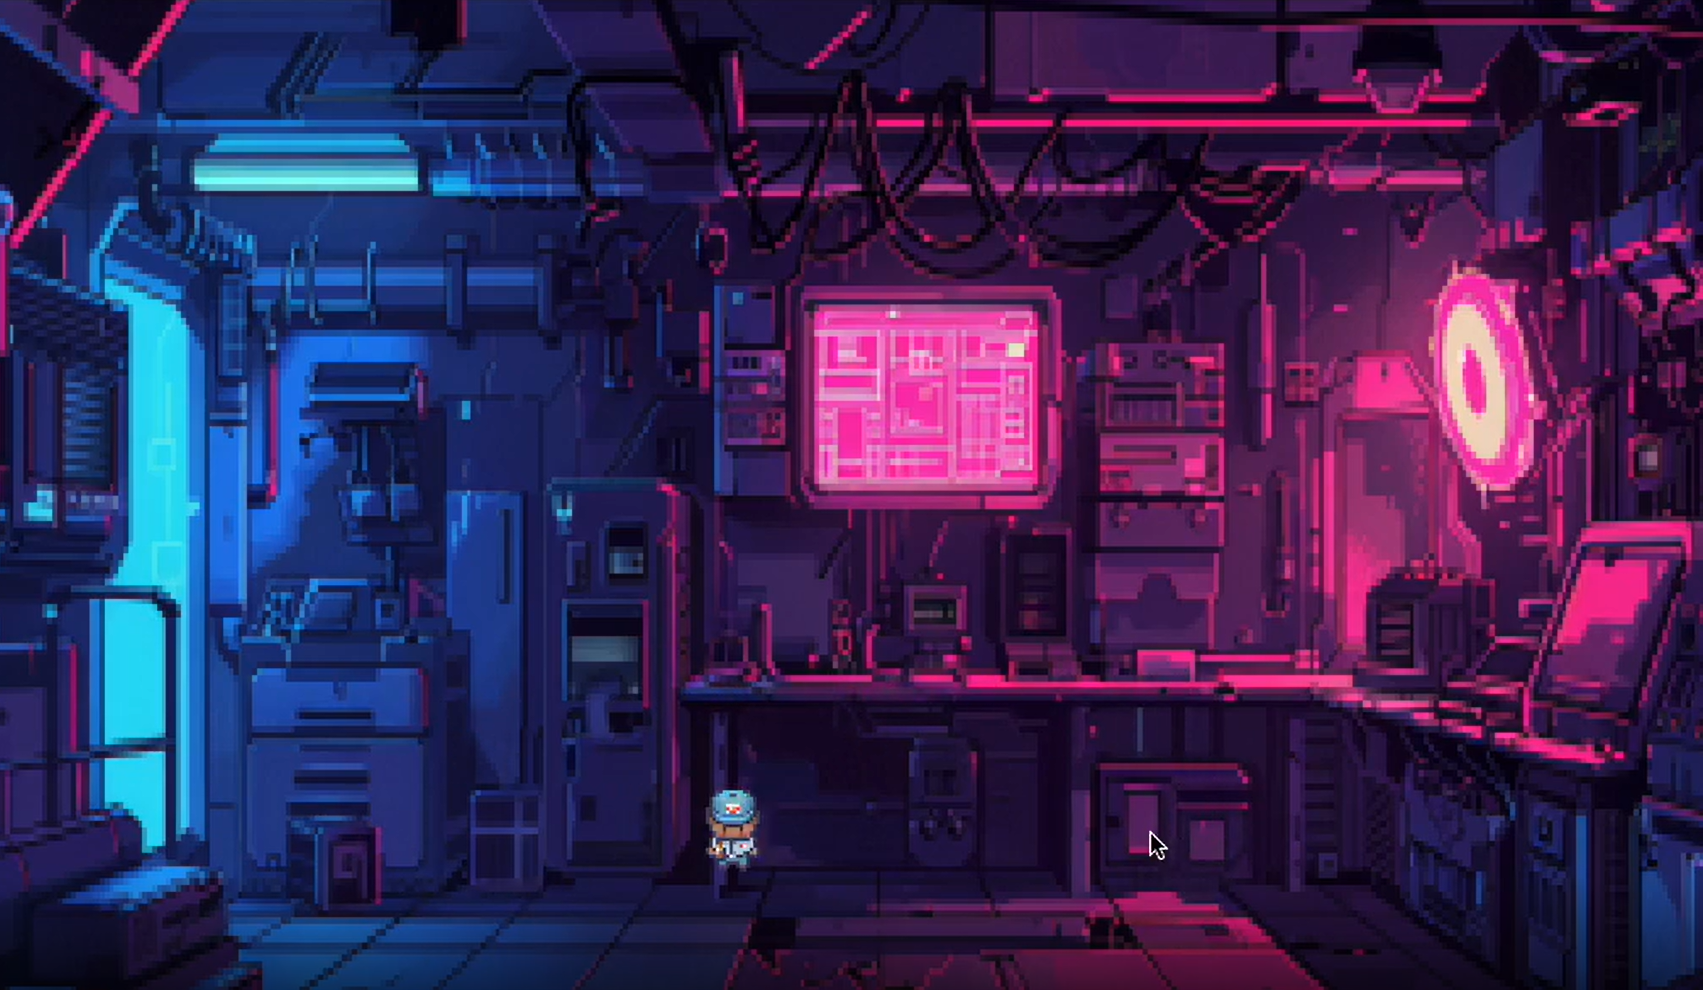
\includegraphics[width=\textwidth]{image/Mockup UI/Player.png}
        \caption*{Player Sprite}
    \end{minipage}
    \hfill
    \begin{minipage}{0.45\textwidth}
        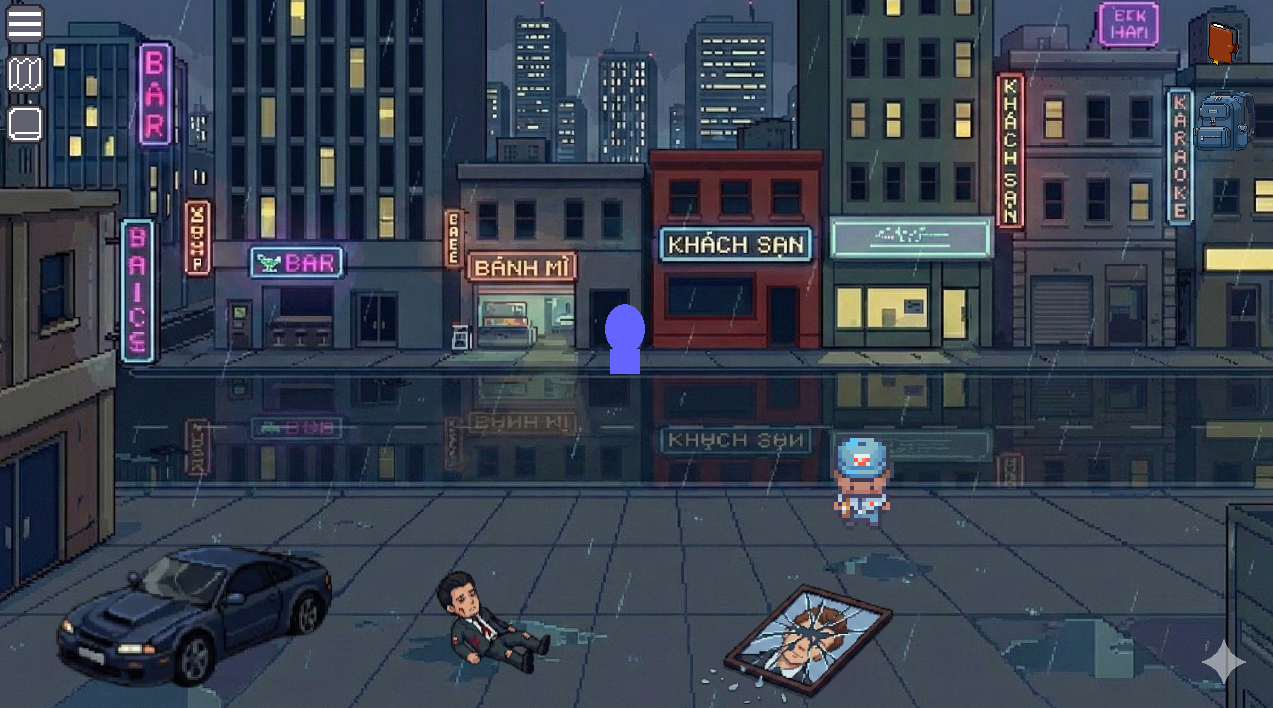
\includegraphics[width=\textwidth]{image/Mockup UI/Player in scene.png}
        \caption*{Player in Environment}
    \end{minipage}

    \vspace{0.5cm}

    % Hàng 2
    \begin{minipage}{0.45\textwidth}
        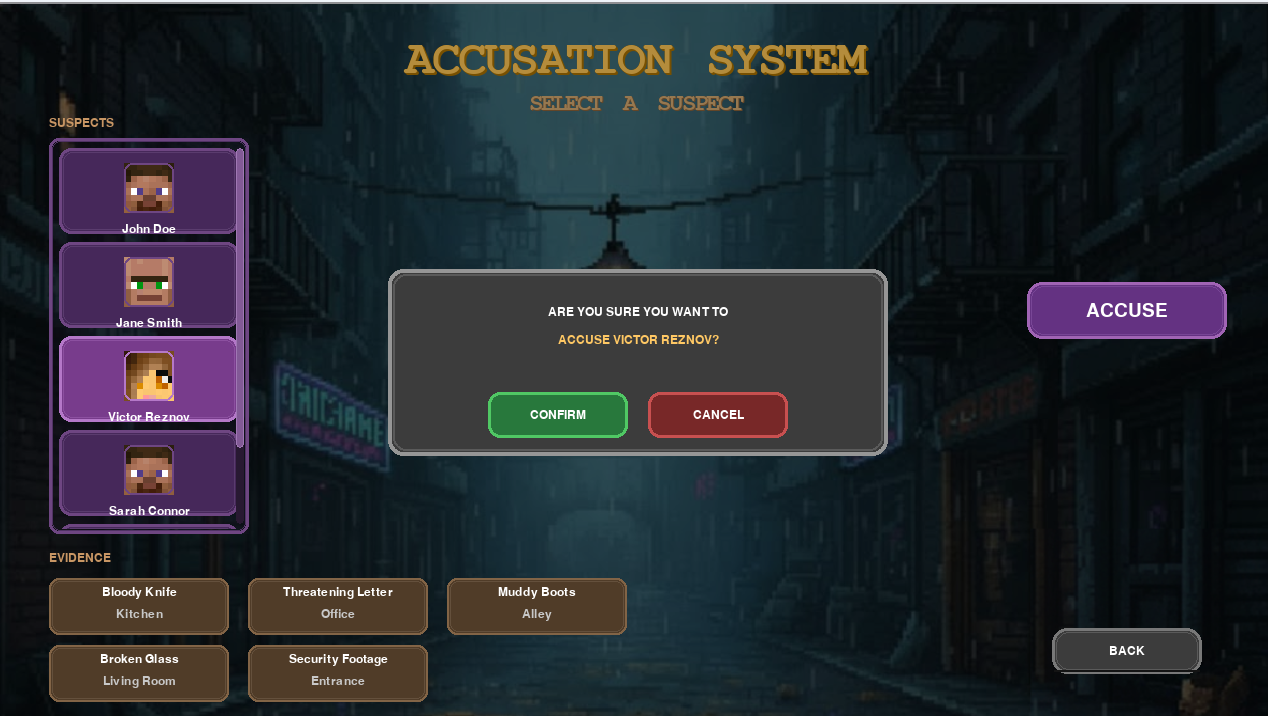
\includegraphics[width=\textwidth]{image/Mockup UI/Accuse.png}
        \caption*{Accusation Interface}
    \end{minipage}
    \hfill
    \begin{minipage}{0.45\textwidth}
        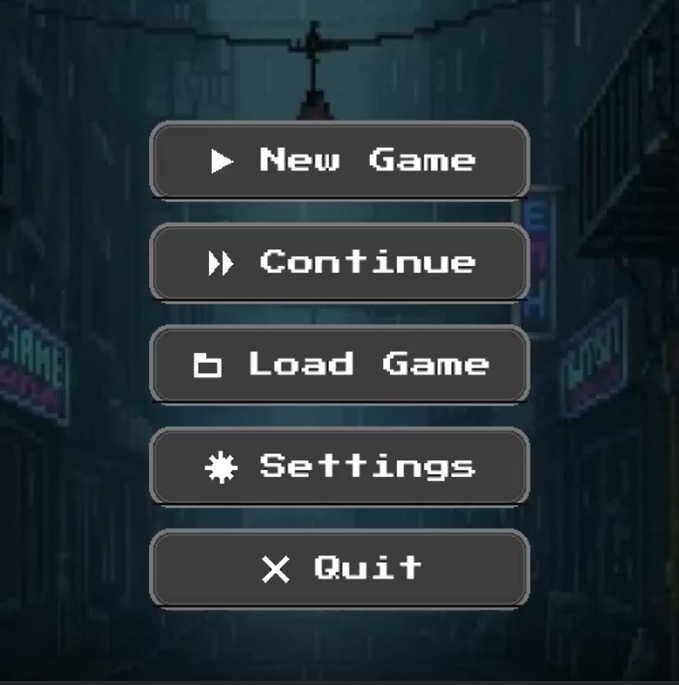
\includegraphics[width=\textwidth]{image/Mockup UI/Button.png}
        \caption*{UI Buttons Assets}
    \end{minipage}
\end{figure}
\clearpage
\section{Mã nguồn dự án}
\href{https://drive.google.com/drive/folders/1G0LLb5vyW6NZmrRqkOVo3SLFaIsprbwf?usp=sharing}{Truy cập vào đây để xem Demo dự án} \\
\href{https://github.com/NghiaNguyenhk2005/DA251}{Truy cập vào đây để xem mã nguồn dự án trên GitHub}

\input{AI}

% \include{References}
% for testing

% % REFERENCES
% \pagebreak
% \nocite{*}
% % Creates references using the Biblatex 
% \bibliographystyle{plain}
% \bibliography{References.bib}
% \newpage
\end{document}